\cleardoublepage
\chapter[Band structures of semiconductors and insulators]{Band structures of semiconductors\break and insulators\label{ch:band-structures}}
In this chapter we discuss the details of practical calculations, and the results obtained for a manifold of reference insulating materials. Thanks to the validity of Bloch's theorem, discussed in \cref{ch:koopmans-periodic}, it is possible to obtain electronic band structures -- within the primitive cell's BZ -- either from a supercell approach, by means of an unfolding method, or from the primitive cell implementation described in \cref{sec:koopmans-pbc}. The computational details of the calculations, including the description of the unfolding method and of the Koopmans workflow, are discussed in \cref{sec:calculations-koopmans}, while in \cref{sec:results-bands} we report the obtained results.

Part of the content of this chapter, as well as the reported results, have been published in Refs.~\cite{de_gennaro_blochs_2022,colonna_koopmans_2022}.

\clearpage
\section{Calculations with Koopmans functionals\label{sec:calculations-koopmans}}
Electronic-structure calculations using Koopmans spectral functionals are performed following two different approaches, based on the two strategies to compute the screening parameters discussed in \cref{sec:screening-parameters}: the first makes use of the finite energy differences strategy and relies on the SC method to model the system deprived of a particle, the second resorts to linear response theory and takes full advantage of the system's symmetries by exploiting the Wannier-like nature of the variational orbitals.

The former represents the original approach used to perform the first calculations in crystalline materials \cite{nguyen_koopmans-compliant_2018}, although, in that case, the quasiparticle energies were computed only at the $\Gamma$-point of the SC (no information about the $\bk$-dispersion). By means of an unfolding technique -- which, once again seizes on the fact that the variational orbitals are WFs, to reconstruct the $\bk$-dependence of the Koopmans Hamiltonian -- here we show, for the very first time, band structures calculations from Koopmans functionals along any path in the BZ \cite{de_gennaro_blochs_2022} (from now on, when speaking of the BZ, we will implicitly refer to the PC's BZ, since the one corresponding to the SC always consists of the $\Gamma$-point only).


The second approach came out more recently \cite{colonna_koopmans_2022} and relies on a second-order approximation of the $\Pi_i$ terms which, for the moment, has been developed only for the KI functional. On the bright side, the linear response approach does not require to compute the self-consistent energies of system with an additional electron or hole -- the screening parameters are computed directly on the neutral system via density-functional perturbation theory (DFPT) -- which makes the calculations much more simple and computationally feasible with respect to the SC approach. Although most of the work carried out in this thesis was performed using the SC approach, in this chapter we will describe also the PC implementation and show some results obtained with this method.

A big part of this thesis was dedicated to the development of some parts of the computational code, to reach a stable implementation working for periodic systems, together with an optimization of the entire workflow required to perform calculations of Koopmans functionals in crystalline materials. In the following sections we give a detailed description of these aspects.


\subsection{Unfolding and interpolation method\label{sec:unfolding-method}}

\begin{equation}
    h^{\rm KC}(\bk,\bk') = \sum_{\bR,\bR'} e^{-i\bk \cdot \bR} e^{i\bk' \cdot \bR'} \braket{w_{\bR} | \hat{h}^{\rm KC}_{\bR'} | w_{\bR'}} .
    \label{eq:double-k-ham}
\end{equation}

When simulating a bulk crystalline material, the infinite system is usually studied with Born-von Karman (BvK) boundary conditions, which introduces a discretization of the $\bk$-points inside the first Brillouin zone (BZ). Equivalently, one can study explicitly the BvK supercell containing the $N$ periodic replicas of the primitive cell, but in this case one no longer has direct access to the band structure of the primitive cell.

In order to recover this band structure, several methods have been developed \cite{boykin_practical_2005, lee_band_2005, ku_unfolding_2010, popescu_extracting_2012, huang_general_2014, medeiros_effects_2014, zheng_quantum_2015}; our approach follows the same strategy of \cite{lee_band_2005} and exploits the Wannier nature of the variational orbitals. The matrix elements of the $\bk$-space Hamiltonian are obtained from those given by the variational orbitals via a (double) Fourier transform as in \cref{eq:double-k-ham}. If the Wannier Hamiltonian is compliant with the translation symmetries of the system, the expression reduces to
%
\begin{equation}
    h^{\rm KC}_{mn}(\bk) = \braket{\psi_{m\bk} | \hat{h}^{\rm KC} | \psi_{n\bk}} = \sum_{\bR} e^{i \bk \cdot \bR} \braket{w_{\bm{0}m} | \hat{h}^{\rm KC}[\rho_{\bR n}] | w_{\bR n}} = \sum_{\bR} e^{i \bk \cdot \bR} h^{\rm KC}_{mn}(\bR) ,
    \label{eq:hk-unfold}
\end{equation}
%
where we have defined $h^{\rm KC}_{mn}(\bR) = \braket{w_{\bm{0}m} | \hat{h}^{\rm KC}[\rho_{\bR n}] | w_{\bR n}}$. The diagonalization of this matrix yields the energies $\varepsilon_{n\bk}$ at any $\bk$-point.

In the supercell approach the Brillouin zone reduces to a single point; as a consequence, the supercell Hamiltonian in the Wannier representation loses the information about the lattice vectors $\{\bR\}$ and its matrix elements are labeled by the supercell index only. In order to reconstruct the $\bk$-space Hamiltonian of \cref{eq:hk-unfold}, one must reconstruct the composite index $\{\bR,n\}$ of each WF from its supercell-picture index ${\alpha}$ (see \cref{fig:map-wf}). An effective way to do this is to first choose a reference primitive cell and define the orbitals with the centers inside it as the $\bR=\bm{0}$ Wannier functions. The second step consists of comparing all the other WFs in the supercell with those in the reference cell. If the Wannier translation property holds, we are able to connect each WF to its reference function $w_{\bm{0} n}$ and lattice vector $\bR$, defined as the distance between the centers of the two functions. If the system has more functions sharing the same center, one can look at the second-order moments ($\braket{x^2}$, $\braket{y^2}$, $\braket{z^2}$) to have a more detailed signature of WFs and, if needed, can move towards higher-order spatial moments until the character of each Wannier function is unequivocally defined \cite{shelley_automated_2011}.

As argued in Ref.~\cite{lee_band_2005}, \cref{eq:hk-unfold} not only applies to the points belonging to the $\bk$-mesh commensurate with the chosen supercell, but it is also an excellent interpolator. So, in order to calculate the band structure along any path in the Brillouin zone, we obtain the matrix elements of the $\bk$-space Hamiltonian by simply applying \cref{eq:hk-unfold} to any arbitrary $\bk$-point. In doing so, the matrix elements $h^{\rm KC}_{mn}(\bR)$, for any $\bR$-vector larger than the supercell are implicitly neglected; the accuracy of the approximation is higher the smaller the contribution from these terms, i.e.\ the more localized the variational orbitals are, or the larger the supercell becomes. A poorly interpolated band structure is usually a symptom of a significant contribution coming from the matrix elements corresponding to larger $\bR$-vectors, and increasing the size of the supercell improves the results.

\begin{figure}
    \centering
    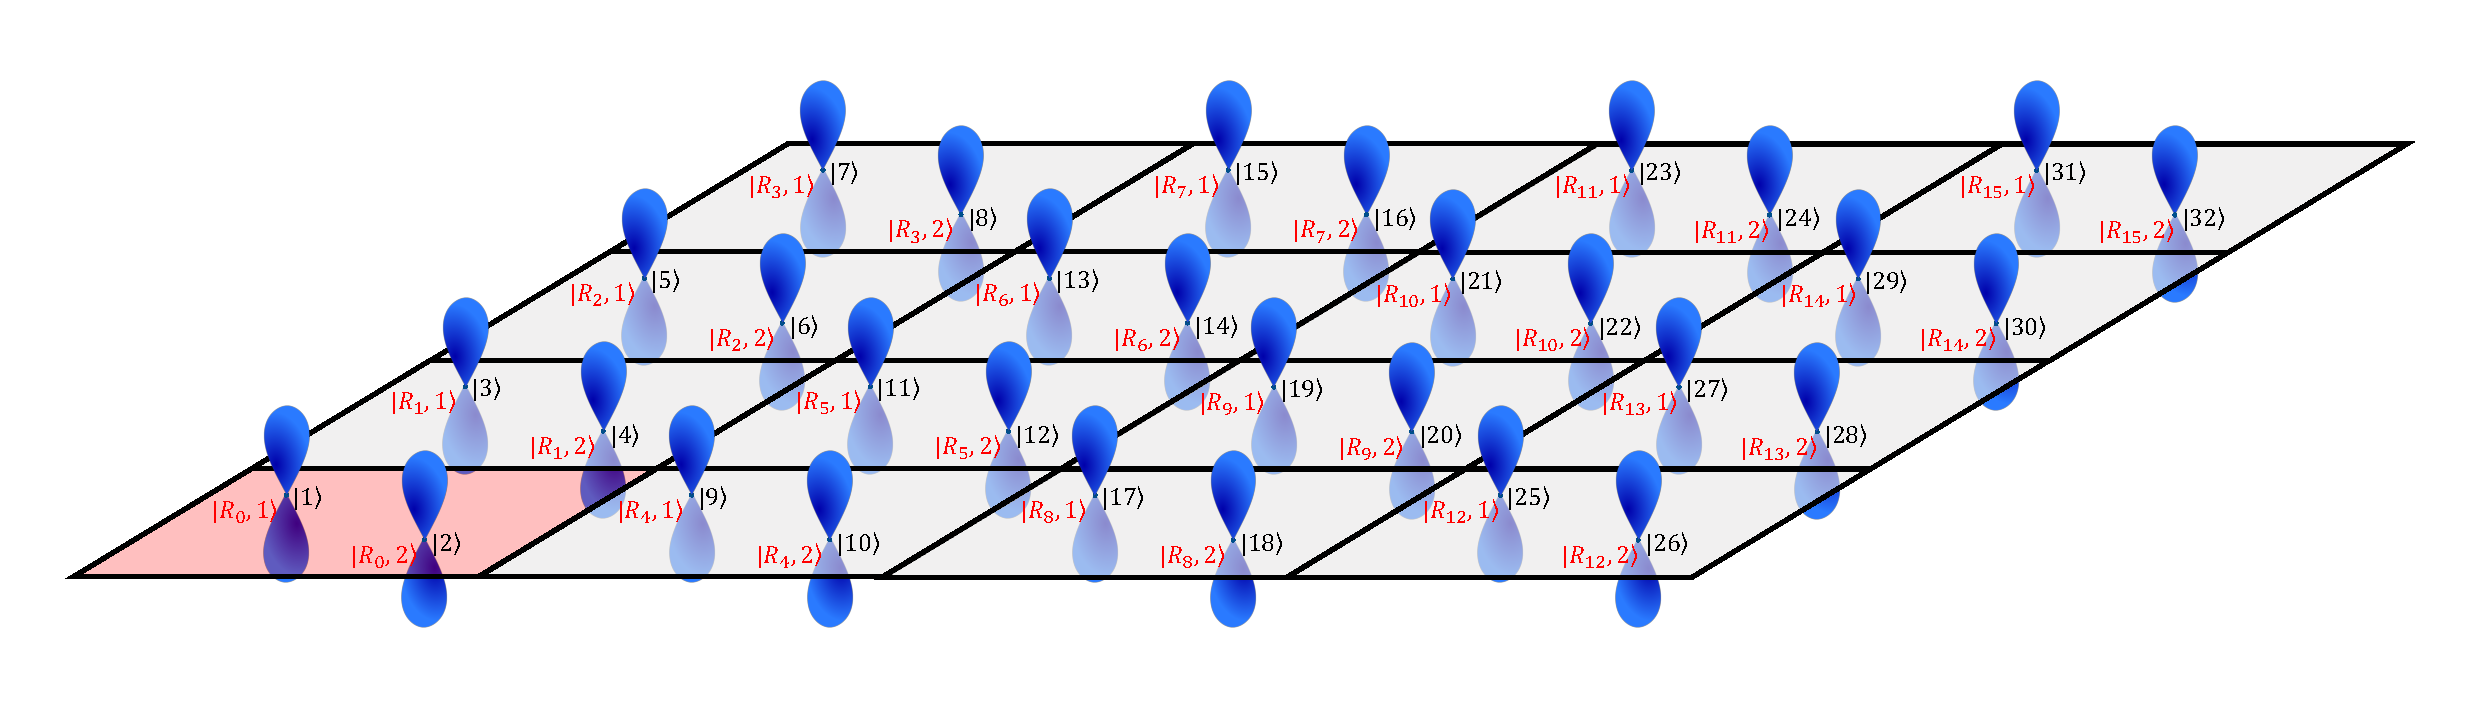
\includegraphics[width=\linewidth]{WF-pcell-scell.pdf}
    \caption[]{Schematic representation of a two-dimensional 2-band model showing the connection between the primitive and supercell Wannier representations. In the primitive picture with a $2\times 2$ sampling of the BZ, the WFs are identified with the pair of labels $\{\bR,n\}$ (red labels): the cell index $\bm{R}$ taking four values and the band index $n$ taking two values. In the $2\times 2$ supercell with $\Gamma$-sampling of the BZ, the eight WFs are labeled by only one quantum number (black labels), i.e.\ the supercell band index $\alpha$ running over the eight states.}
    \label{fig:map-wf}
\end{figure}


\subsection{Workflow\label{sec:workflow}}

\begin{figure}
    \centering
    \subfloat[]{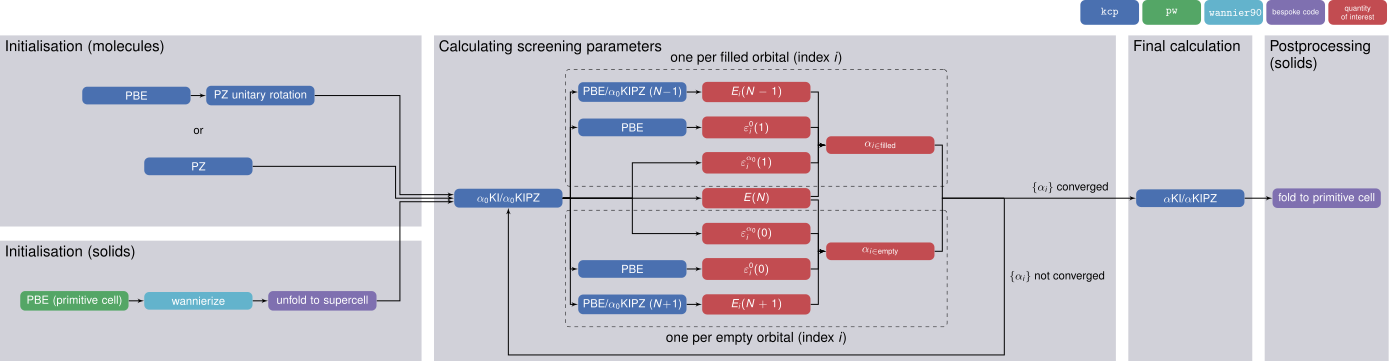
\includegraphics[width=\linewidth]{dscf_workflow.png}} \\
    \subfloat[]{
\includegraphics[width=\linewidth]{dfpt_workflow.png}}
    \caption[]{}
    \label{fig:workflow}
\end{figure}

\subsection{Computational details\label{sec:computational-details}}

\section{Results\label{sec:results-bands}}

\subsection{Finite differences\label{sec:results-dscf}}

\subsection{DFPT\label{sec:results-dfpt}}

